\chapter{Marco Teórico}

% En este capítulo, se presenta las principales tecnologías de detección en primer  plano del objeto en movimiento, descripción y extracción de características,  clasificación y reconocimiento del movimiento humano. Basado en el flujo óptico para la detección de objetos en movimiento. Como también la imagen de flujo de energía óptico para la detección de características de movimiento y se adoptaron redes neuronales convolucionales de región para elegir  características y reducir la dimensión. Luego, gracias al clasificador de máquina de vectores de soporte que puede ser entrenado y utilizado para clasificar y reconocer acciones; es posible distinguir efectivamente las acciones humanas y mejorar significativamente la precision del reconocimineto de las acciones humanas.

\section{Sistema de video vigilancia}
La videovigilancia consiste en la instalción de cámaras de vídeo que sirven como grabadoras las cuales guardan su contenido en un almacén digital el cual puede ser visto en un monitor central. Un sistema de video vigilancia es una instalación de seguridad cuya finalidad es el control y supervisión visual en tiempo real de instalaciones locales y remotas, mediante el uso de múltiples cámaras de vigilancia, así como de sistemas de visualización, grabación y archivo. Estos sistemas ayudan a proteger a las personas, bienes y recursos, mantienen la alerta y poseen un gran efecto disuasorio \cite{wikipedia:vvigilancia}.\\

Estos sistemas capturan imágenes y vídeos, que pueden ser comprimidos, almacenados, o enviados por una red de comunicación y pueden ser instalados en cualquier ambiente. En la figura \ref{fig:sistema_video_vigilancia} se visualiza la composición de un sistema de video vigilancia actual. Este sistema compone de un conjunto de cámaras que estan conectados directamente a un (NVR - Network Video Recorder) grabador de video en red, el cual permite la visualización de lo que las cámaras estan captando en un monitor local y por medio de una conección a un punto de acceso a internet, permite la visualización de esta transmisión en dispositivos externos a la red local\\.

\begin{figure}[H]
    \begin{center}
        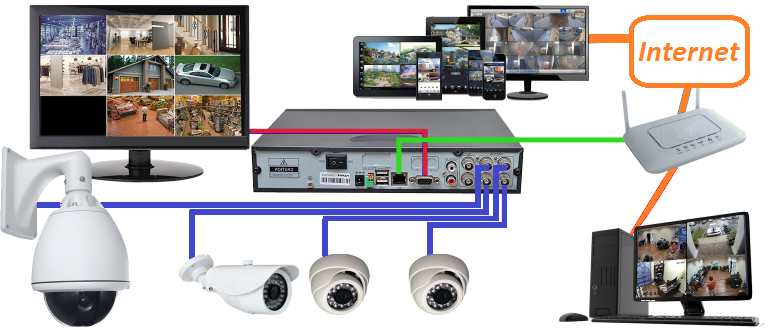
\includegraphics[width=9cm]{img/capitulo_2/sis_videovigilancia.png}
    \end{center}
    \caption{Sistema actual de videovigilancia\\Fuente: Web}
    \label{fig:sistema_video_vigilancia}
\end{figure}

A continuación se detalla los componentes que forman parte del prototipo del sistema de video vigilancia inteligente propuesto.

% Sistemas de videovigilancia inteligente La técnica clave del reconocimiento de la accion humana basada en la vision  por compoutadora consiste en describir y comprender los comportamientos humanos por medio de la vision por computadora.\\

% Este proceso es una tarea complicada e integra algunos campos de investigacion que incluyen el procesamiento de imagen, aperndizaje automatico, reconocimiento de patrones, etc.\\

% La detección de un objeto móvil consiste en separar las áreas de cambio en el video es decir en las imádgenes de fondo que comprenden el video, dicho de otra manera, separar correctamente las áreas y contornos del objetico movil. Es critico para el siguiente procesamiento la segementación efectiva \\



\section{Visión por Computadora}

\section{Redes Neuronales}

\section{Protocolos de red IP/HTTP}

\subsection{TCP/IP}

\subsection{HTTP}

\section{Video Streaming}

\subsection{Formatos}

\subsubsection{HLS}

\subsubsection{DASH}

\section{Metodología de desarrollo}
